\subsection{UC1 - Autenticazione}
\begin{figure}[H]
    \centering
    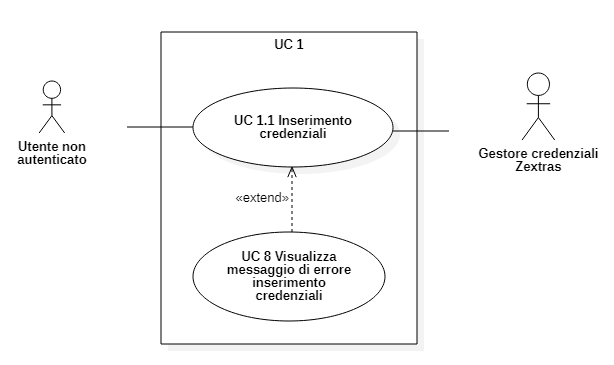
\includegraphics[scale = 0.7]{components/img/UC1.png}
    \caption{UC1 - Autenticazione}
\end{figure}
\subsubsection{UC1.1 - Inserimento credenziali}
\begin{itemize}
\item \textbf{Attore Primario:} Utente non autenticato;
\item \textbf{Attore Secondario:} Gestore credenziali Zextras;
\item \textbf{Precondizione:} L'utente non è riconosciuto dal \glo{sistema};
\item \textbf{Postcondizione:} L'utente ha effettuato il login usando le credenziali di \glo{Zextras Drive};
\item \textbf{Scenario principale:}
    \begin{enumerate}
    \item L'utente avvia l'applicazione per la prima volta;
    \item L'utente inserisce le credenziali relative al suo account \glo{Zextras Drive};
    \end{enumerate}
\item \textbf{Estensioni:}
\begin{itemize}
\item Visualizza messaggio di errore inserimento credenziali (UC8 \S{}\ref{UC8}).
\end{itemize}
\end{itemize}
